% !TeX root = ../../Nucleation in the Ising Model.tex
    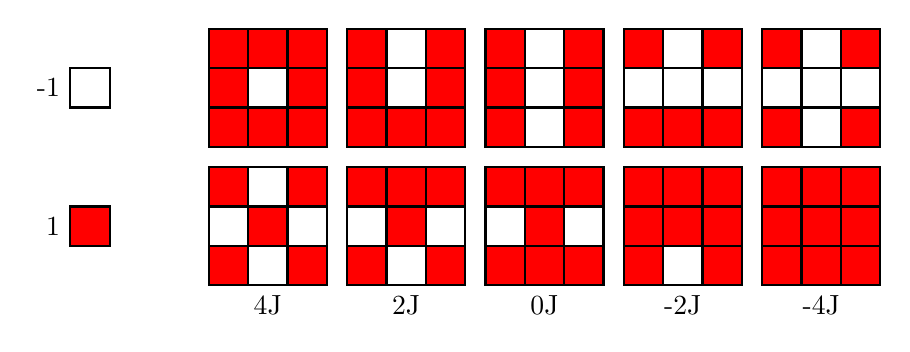
\begin{tikzpicture}[thick,>=latex,scale=1,l/.style={latex-latex},F/.style={-latex,very thick},v/.style={-latex',thick},
			vc/.style={-latex',thick,color=gray},d/.style={thin},w/.style={fill=white}] 

\begin{scope}[xshift=-50]
	\filldraw[draw=black, fill=red](0,0.5)rectangle+(0.5,0.5);\draw(0,0.75)node[left]{1};
\begin{scope}[yshift=50]
	\filldraw[draw=black,fill=white](0,0.5)rectangle+(0.5,0.5);\draw(0.0,0.75)node[left]{-1};
\end{scope}
\end{scope}


\visible<1->{
\begin{scope}
\foreach \i in {0, 0.5, ..., 1.5} {
	\draw(0,\i)--+(1.5,0);
	\draw(\i,0)--+(0,1.5);
 }
\filldraw[draw=black, fill=red](0.5,0.5)rectangle+(0.5,0.5);

\visible<6->{
	\filldraw[draw=black, fill=red](1,1)rectangle+(0.5,0.5);
	\filldraw[draw=black, fill=red](0.0,0)rectangle+(0.5,0.5);
	\filldraw[draw=black, fill=red](1,0)rectangle+(0.5,0.5);
	\filldraw[draw=black, fill=red](0,1)rectangle+(0.5,0.5);
}
\draw(0.75,0)node[below]{4J};
\begin{scope}[yshift=50]
\foreach \i in {0, 0.5, ..., 1.5} {
	\draw(0,\i)--+(1.5,0);
	\draw(\i,0)--+(0,1.5);
 }
\filldraw[draw=black, fill=red](1,1)rectangle+(0.5,-0.5);
\filldraw[draw=black, fill=red](0.5,1)rectangle+(0.5,0.5);
\filldraw[draw=black, fill=red](1,0)rectangle+(-0.5,0.5);
\filldraw[draw=black, fill=red](0,1)rectangle+(0.5,-0.5);


\visible<6->{
	\filldraw[draw=black, fill=red](1,1)rectangle+(0.5,0.5);
	\filldraw[draw=black, fill=red](0.0,0)rectangle+(0.5,0.5);
	\filldraw[draw=black, fill=red](1,0)rectangle+(0.5,0.5);
	\filldraw[draw=black, fill=red](0,1)rectangle+(0.5,0.5);
}

\end{scope}
\end{scope}

}\visible<2->{


\begin{scope}[xshift=50]
\foreach \i in {0, 0.5, ..., 1.5} {
	\draw(0,\i)--+(1.5,0);
	\draw(\i,0)--+(0,1.5);
 }
\filldraw[draw=black, fill=red](0.5,0.5)rectangle+(0.5,0.5);
\filldraw[draw=black, fill=red](0.5,1)rectangle+(0.5,0.5);%1


\visible<6->{
	\filldraw[draw=black, fill=red](1,1)rectangle+(0.5,0.5);
	\filldraw[draw=black, fill=red](0.0,0)rectangle+(0.5,0.5);
	\filldraw[draw=black, fill=red](1,0)rectangle+(0.5,0.5);
	\filldraw[draw=black, fill=red](0,1)rectangle+(0.5,0.5);
}

\draw(0.75,0)node[below]{2J};
\begin{scope}[yshift=50]
\foreach \i in {0, 0.5, ..., 1.5} {
	\draw(0,\i)--+(1.5,0);
	\draw(\i,0)--+(0,1.5);
 }

%\filldraw[draw=black, fill=red](0.5,1)rectangle+(0.5,0.5);%1
\filldraw[draw=black, fill=red](1,1)rectangle+(0.5,-0.5);%2
\filldraw[draw=black, fill=red](1,0)rectangle+(-0.5,0.5);%3
\filldraw[draw=black, fill=red](0,1)rectangle+(0.5,-0.5);%4


\visible<6->{
	\filldraw[draw=black, fill=red](1,1)rectangle+(0.5,0.5);
	\filldraw[draw=black, fill=red](0.0,0)rectangle+(0.5,0.5);
	\filldraw[draw=black, fill=red](1,0)rectangle+(0.5,0.5);
	\filldraw[draw=black, fill=red](0,1)rectangle+(0.5,0.5);
}

\end{scope}
\end{scope}
}\visible<3->{


\begin{scope}[xshift=100]
\foreach \i in {0, 0.5, ..., 1.5} {
	\draw(0,\i)--+(1.5,0);
	\draw(\i,0)--+(0,1.5);
 }
\filldraw[draw=black, fill=red](0.5,1)rectangle+(0.5,0.5);%1
\filldraw[draw=black, fill=red](0.5,0.5)rectangle+(0.5,0.5);
\filldraw[draw=black, fill=red](1,0)rectangle+(-0.5,0.5);%3

\visible<6->{
	\filldraw[draw=black, fill=red](1,1)rectangle+(0.5,0.5);
	\filldraw[draw=black, fill=red](0.0,0)rectangle+(0.5,0.5);
	\filldraw[draw=black, fill=red](1,0)rectangle+(0.5,0.5);
	\filldraw[draw=black, fill=red](0,1)rectangle+(0.5,0.5);
}

\draw(0.75,0)node[below]{0J};
\begin{scope}[yshift=50]
\foreach \i in {0, 0.5, ..., 1.5} {
	\draw(0,\i)--+(1.5,0);
	\draw(\i,0)--+(0,1.5);
 }
%\filldraw[draw=black, fill=red](0.5,1)rectangle+(0.5,0.5);%1
\filldraw[draw=black, fill=red](1,1)rectangle+(0.5,-0.5);%2
%\filldraw[draw=black, fill=red](1,0)rectangle+(-0.5,0.5);%3
\filldraw[draw=black, fill=red](0,1)rectangle+(0.5,-0.5);%4

\visible<6->{
	\filldraw[draw=black, fill=red](1,1)rectangle+(0.5,0.5);
	\filldraw[draw=black, fill=red](0.0,0)rectangle+(0.5,0.5);
	\filldraw[draw=black, fill=red](1,0)rectangle+(0.5,0.5);
	\filldraw[draw=black, fill=red](0,1)rectangle+(0.5,0.5);
}

\end{scope}
\end{scope}

}\visible<4->{

\begin{scope}[xshift=150]
\foreach \i in {0, 0.5, ..., 1.5} {
	\draw(0,\i)--+(1.5,0);
	\draw(\i,0)--+(0,1.5);
 }
\filldraw[draw=black, fill=red](0.5,0.5)rectangle+(0.5,0.5);
\filldraw[draw=black, fill=red](0.5,1)rectangle+(0.5,0.5);%1
\filldraw[draw=black, fill=red](1,1)rectangle+(0.5,-0.5);%2
%\filldraw[draw=black, fill=red](1,0)rectangle+(-0.5,0.5);%3
\filldraw[draw=black, fill=red](0,1)rectangle+(0.5,-0.5);%4


\visible<6->{
	\filldraw[draw=black, fill=red](1,1)rectangle+(0.5,0.5);
	\filldraw[draw=black, fill=red](0.0,0)rectangle+(0.5,0.5);
	\filldraw[draw=black, fill=red](1,0)rectangle+(0.5,0.5);
	\filldraw[draw=black, fill=red](0,1)rectangle+(0.5,0.5);
}

\draw(0.75,0)node[below]{-2J};
\begin{scope}[yshift=50]
\foreach \i in {0, 0.5, ..., 1.5} {
	\draw(0,\i)--+(1.5,0);
	\draw(\i,0)--+(0,1.5);
 }


\visible<6->{
	\filldraw[draw=black, fill=red](1,1)rectangle+(0.5,0.5);
	\filldraw[draw=black, fill=red](0.0,0)rectangle+(0.5,0.5);
	\filldraw[draw=black, fill=red](1,0)rectangle+(0.5,0.5);
	\filldraw[draw=black, fill=red](0,1)rectangle+(0.5,0.5);
}

%\filldraw[draw=black, fill=red](0.5,1)rectangle+(0.5,0.5);%1
%\filldraw[draw=black, fill=red](1,1)rectangle+(0.5,-0.5);%2
\filldraw[draw=black, fill=red](1,0)rectangle+(-0.5,0.5);%3
%\filldraw[draw=black, fill=red](0,1)rectangle+(0.5,-0.5);%4
\end{scope}
\end{scope}
}\visible<5->{

\begin{scope}[xshift=200]
\foreach \i in {0, 0.5, ..., 1.5} {
	\draw(0,\i)--+(1.5,0);
	\draw(\i,0)--+(0,1.5);
 }


\visible<6->{
	\filldraw[draw=black, fill=red](1,1)rectangle+(0.5,0.5);
	\filldraw[draw=black, fill=red](0.0,0)rectangle+(0.5,0.5);
	\filldraw[draw=black, fill=red](1,0)rectangle+(0.5,0.5);
	\filldraw[draw=black, fill=red](0,1)rectangle+(0.5,0.5);
}

\filldraw[draw=black, fill=red](0.5,0.5)rectangle+(0.5,0.5);
\filldraw[draw=black, fill=red](0.5,1)rectangle+(0.5,0.5);%1
\filldraw[draw=black, fill=red](1,1)rectangle+(0.5,-0.5);%2
\filldraw[draw=black, fill=red](1,0)rectangle+(-0.5,0.5);%3
\filldraw[draw=black, fill=red](0,1)rectangle+(0.5,-0.5);%4
\draw(0.75,0)node[below]{-4J};
\begin{scope}[yshift=50]
\foreach \i in {0, 0.5, ..., 1.5} {
	\draw(0,\i)--+(1.5,0);
	\draw(\i,0)--+(0,1.5);
 }
%\filldraw[draw=black, fill=red](0.5,1)rectangle+(0.5,0.5);%1
%\filldraw[draw=black, fill=red](1,1)rectangle+(0.5,-0.5);%2
%\filldraw[draw=black, fill=red](1,0)rectangle+(-0.5,0.5);%3
%\filldraw[draw=black, fill=red](0,1)rectangle+(0.5,-0.5);%4


\visible<6->{
	\filldraw[draw=black, fill=red](1,1)rectangle+(0.5,0.5);
	\filldraw[draw=black, fill=red](0.0,0)rectangle+(0.5,0.5);
	\filldraw[draw=black, fill=red](1,0)rectangle+(0.5,0.5);
	\filldraw[draw=black, fill=red](0,1)rectangle+(0.5,0.5);
}

\end{scope}
\end{scope}
}
    \end{tikzpicture}